\documentclass[sigconf,nonacm]{acmart}
\settopmatter{printacmref=false}
\setcopyright{none}
\usepackage{booktabs}
\usepackage{graphicx}
\usepackage{microtype}
\graphicspath{{images/}}
\title{SynVulCommit: Validated LLM-Based Synthetic Commit Generation for Python Vulnerability Detection}
\author{Wassim Bejaoui}
\affiliation{\institution{University of Passau}\department{Faculty of Computer Science and Mathematics}\city{Passau}\country{Germany}}
\email{wassim.bejaoui@uni-passau.de}
\author{Sofian Yadir}
\affiliation{\institution{University of Passau}\department{Faculty of Computer Science and Mathematics}\city{Passau}\country{Germany}}
\email{sofian.yadir@uni-passau.de}
\begin{document}
\begin{abstract}
Machine-learning vulnerability detection depends on labeled code corpora, but real vulnerability-fixing commits are costly to mine and difficult to balance across weakness categories. This paper presents SynVulCommit, a provider-agnostic pipeline for generating Python vulnerability-fix commit pairs across seven VUDENC-compatible Common Weakness Enumeration (CWE) categories. The pipeline combines deterministic quota planning, CWE-specific structural checks, Bandit and Semgrep analysis, a second-stage large language model (LLM) reviewer, and exact, abstract-syntax-tree, and token-shingle duplicate rejection. The final verified window-balanced corpus contains 1,205 accepted pairs. From this corpus we freeze a balanced 1,043-pair subset with 149 synthetic commits per CWE and compare it with real VUDENC data under three training conditions: real-only, synthetic-only, and mixed real-plus-synthetic. We evaluate eight model variants from the previous labs: LSTM, multilayer perceptron (MLP), Random Forest, and convolutional neural network (CNN) with Word2Vec features, plus LSTM and CNN variants with CodeBERT and GraphCodeBERT embeddings. All models are evaluated on the same held-out real VUDENC test split. Synthetic-only training remains weaker than real-only training, showing that validated synthetic commits do not automatically match the real-data distribution. However, mixed training improves the best MLP result to a mean macro-F1 of 0.7161, the strongest overall score. These results support SynVulCommit as a controlled data-generation and augmentation framework, while showing that validation, diversity, and downstream representation must be designed together.
\end{abstract}
\maketitle
\begin{abstract}
Machine-learning vulnerability detection depends on labeled code corpora, but real vulnerability-fixing commits are expensive to mine and difficult to balance across weakness categories. This paper presents SynVulCommit, a provider-agnostic pipeline for generating Python vulnerability-fix commit pairs across seven VUDENC-compatible Common Weakness Enumeration (CWE) categories. The pipeline combines deterministic quota planning, CWE-specific structural checks, Bandit and Semgrep analysis, a second-stage large language model (LLM) reviewer, and exact, abstract-syntax-tree, and token-based duplicate rejection. It produced 678 accepted pairs. A frozen 637-pair subset, balanced at 91 pairs per CWE, was compared with real VUDENC data using LSTM, multilayer perceptron (MLP), Random Forest, and convolutional neural network (CNN) models with shared Word2Vec features. All conditions were evaluated on the same held-out real VUDENC commits. Real-only training achieved the strongest mean macro-F1, led by Random Forest at 0.6618. Synthetic-only training was substantially weaker, primarily because compact generated files created a strongly positive-skewed window representation. Combining real and synthetic data improved the LSTM slightly but did not improve the other three models. The result supports using validated synthetic commits for controlled data-generation research, while showing that generation quality alone does not remove representation and distribution-shift risks.
\end{abstract}

\section{Introduction}
Software vulnerabilities remain a high-impact source of security failures, and source-code learning methods are increasingly used to prioritize or classify vulnerable code. Their effectiveness depends on the quality, coverage, and labeling discipline of training data. Real repositories provide valuable examples, but vulnerability-fixing commits are sparse, noisy, and unevenly distributed across weakness types. VUDENC addresses this problem for Python by deriving vulnerable and fixed code from natural vulnerability-fixing commits \cite{vudenc}. However, a mined corpus cannot guarantee uniform coverage of a chosen CWE, framework, program structure, or data-flow pattern.

This work investigates whether an LLM can generate useful, commit-like Python vulnerability data while maintaining a strong validation boundary. SynVulCommit produces paired vulnerable and fixed files rather than isolated snippets. The objective is not to claim that LLM-generated data replaces real commits. Instead, the system creates a controlled corpus that supports an explicit experiment: compare models trained on real data, synthetic data, and their combination using a shared real-data test set.

The contributions are:
\begin{enumerate}
  \item A generation pipeline for seven Python CWE categories with deterministic quota-based coverage over application type, flow pattern, difficulty, and program structure.
  \item A layered acceptance policy combining CWE-specific structural checks, Bandit, Semgrep, a blinded LLM reviewer, and near-duplicate rejection.
  \item A clean VUDENC-style training export and a separate sanitized audit sidecar.
  \item A controlled A/B/C evaluation using four Word2Vec-based model families and a fixed held-out real VUDENC test split.
\end{enumerate}

\section{Background and Related Work}
Deep learning for vulnerability detection has progressed from code-gadget and representation-learning approaches, such as VulDeePecker \cite{vuldeepecker} and early deep representation learning \cite{russell2018}, to systematic vulnerability representations \cite{sysevr} and graph-based program semantics \cite{devign}. Dataset construction remains central: Big-Vul demonstrates the value of commit-level vulnerability data with code changes and CVE summaries \cite{bigvul}, while VUDENC specifically provides a Python corpus based on natural vulnerable/fixed commits \cite{vudenc}. Reviews of the area caution that reported performance can depend strongly on dataset construction and evaluation setup \cite{chakraborty2022}.

Pre-trained code models offer richer representations. CodeBERT jointly pre-trains on programming and natural-language data \cite{codebert}; GraphCodeBERT adds data-flow structure \cite{graphcodebert}; and VulBERTa targets vulnerability detection through simplified source-code pre-training \cite{vulberta}. In Lab 3, Word2Vec CNN models were more stable than the CodeBERT and GraphCodeBERT experiments, especially for SQL injection. Therefore, this paper uses the four established Word2Vec model families as the primary comparison and treats transformer results as prior context rather than mixing different training protocols.

LLMs can both assist development and introduce risks. Pearce et al. found insecure code patterns in generated Copilot suggestions \cite{pearce2022}. Conversely, LLM-based augmentation has been studied for long-tail vulnerability detection \cite{deng2024}. These findings motivate a conservative design: LLMs propose candidates, but deterministic analysis and independent review decide whether candidates enter the corpus.

\section{SynVulCommit Methodology}
\subsection{Generation Scope and Quota Planning}
The pipeline targets SQL injection (CWE-89), command injection (CWE-78), path traversal (CWE-22), open redirect (CWE-601), remote code execution (CWE-94), cross-site scripting (CWE-79), and cross-site request forgery (CWE-352). For each requested sample, a deterministic planner selects a compatible tuple of application type, data-flow pattern, difficulty, and structure. The planner favors the least-represented full tuple, then the least-represented marginal values, with a stable SHA-256 tie-breaker. A rejected candidate retries the same planned slot; it is not replaced by a random context.

The LLM returns a strict JSON object containing a commit message, relative filename, vulnerable code, fixed code, and exact changed lines. The prompt requires one requested CWE, a behavior-preserving fix, and no unrelated security-sensitive flow. Provider configuration is externalized through environment variables; keys, endpoints, raw replies, and authorization data are never stored in training exports.

\subsection{Validation and Review}
Figure~\ref{fig:pipeline} summarizes the acceptance path. Structural checks verify the intended source, sink, framework context, and fix strategy. Bandit and Semgrep then analyze vulnerable and fixed files. The requested rule must appear before the fix where configured, and no configured SynVulCommit CWE rule may remain after the fix. This cross-CWE post-fix rule prevents, for example, accepting an XSS fix that introduces SQL injection.

\begin{figure*}[t]
\centering
\fbox{\parbox{0.92\textwidth}{
\centering
\textbf{Quota-planned specification} $\rightarrow$ \textbf{LLM commit pair} $\rightarrow$ \textbf{structural checks} $\rightarrow$ \textbf{Bandit and Semgrep} $\rightarrow$ \textbf{blinded LLM review} $\rightarrow$ \textbf{duplicate policy} $\rightarrow$ \textbf{accepted JSONL and VUDENC export}

\vspace{0.6em}
Rejected candidates retry the same quota slot. Accepted records preserve detailed internal audit data; the training export contains only code, diffs, and changed fragments.
}}
\caption{SynVulCommit generation and acceptance pipeline.}
\label{fig:pipeline}
\end{figure*}

After deterministic validation, a second-stage reviewer receives the requested CWE/context and the vulnerable/fixed code, but not analyzer output or provider metadata. It returns a strict structured verdict. A candidate is accepted only when the review status is complete and the verdict is \texttt{pass}. This is a quality gate, not a replacement for static analysis.

\subsection{Diversity, Export, and Verification}
The diversity index rejects candidates in policy order: exact normalized vulnerable/fixed pair hashes, normalized AST-pair fingerprints, and same-CWE token-shingle similarity at Jaccard similarity at least 0.90. AST normalization removes identifiers, names, aliases, attributes, keywords, and literal-specific variation, preventing superficial renaming from creating a new sample.

Accepted records are exported to \texttt{plain\_<mode>} VUDENC-style files. These files retain only the commit message, vulnerable/fixed sources, diff, filename, add/remove counts, \texttt{badparts}, and \texttt{goodparts}. The separate \texttt{metadata.jsonl} sidecar contains sanitized provenance and validation summaries. A strict dataset verifier checks the accepted records, rejected categories, duplicate policy, reviewer state, and exact linkage between JSONL records and exported commits.

\section{Experimental Design}
\subsection{Datasets and Splits}
The accepted generation output contained 678 pairs. Figure~\ref{fig:coverage} shows the per-CWE counts. To avoid selecting a stronger CWE merely because it had more generated candidates, the experiment froze 91 synthetic pairs per CWE, for 637 pairs total. The selection was deterministic and stratified by the four generation context dimensions.

\begin{figure}[t]
\centering
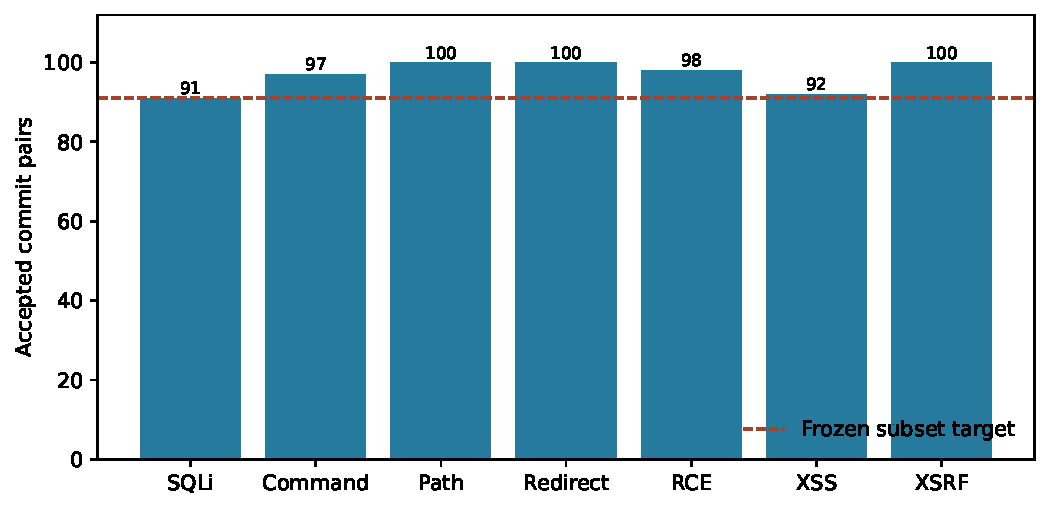
\includegraphics[width=\linewidth]{corpus_coverage.pdf}
\caption{Accepted pairs in the source corpus. The dashed line marks the 91-pair-per-CWE frozen subset used for evaluation.}
\label{fig:coverage}
\end{figure}

Real VUDENC data was normalized into the same commit-level representation; legacy \texttt{path\_disclosure} was mapped to \texttt{directory\_traversal}. The real cap was $\min(91, \text{available commits})$ per CWE. Remote code execution had 54 available real commits and XSS had 69; the remaining CWEs had 91 selected commits. Commits, not windows, were deterministically split approximately 70/15/15 into train/validation/test. Consequently, every window from a multi-file commit stays in one split.

Windows contain up to 200 lexical code tokens. A vulnerable-source window overlapping a \texttt{badpart} is labeled vulnerable; other source windows are labeled clean. For computational tractability, each file retains at most four positive and four negative windows. This preserves the original source-window semantics but creates an important limitation for compact generated files, discussed in Section~\ref{sec:discussion}.

\subsection{A/B/C Conditions and Models}
Condition A trains and validates on real VUDENC data. Condition B trains and validates on the synthetic subset. Condition C trains on their union and validates on real VUDENC. Every condition is evaluated on the identical held-out real VUDENC test set. The real train/validation/test window counts were 5,286/1,083/1,143; synthetic counts were 513/104/114, although synthetic test windows were not used.

All models use a shared independently trained 300-dimensional Python Word2Vec representation. The saved legacy Word2Vec metadata file lacked its vector sidecar, so the model was rebuilt from the existing external Python corpus and stored inside the experiment release. The evaluated models were:
\begin{itemize}
  \item LSTM: 100 units and 0.2 dropout;
  \item MLP: 256 and 128 ReLU hidden units with Adam;
  \item Random Forest: 300 trees and balanced class weights;
  \item CNN: 128 one-dimensional filters, kernel size 5, global max pooling, dense 128, and 0.2 dropout.
\end{itemize}
Sequence models use 200 token IDs with fixed Word2Vec embeddings. MLP and Random Forest use mean-pooled 300-dimensional vectors. Neural models use Adam, batch size 128, up to 100 epochs, and early stopping based on validation F1. Python, NumPy, scikit-learn, and TensorFlow seeds are fixed.

\section{Results}
Figure~\ref{fig:abc} reports the mean macro-F1 across the seven CWEs. Macro-F1 is emphasized because a high vulnerable-class recall can hide a model that predicts most windows as vulnerable.

\begin{figure}[t]
\centering
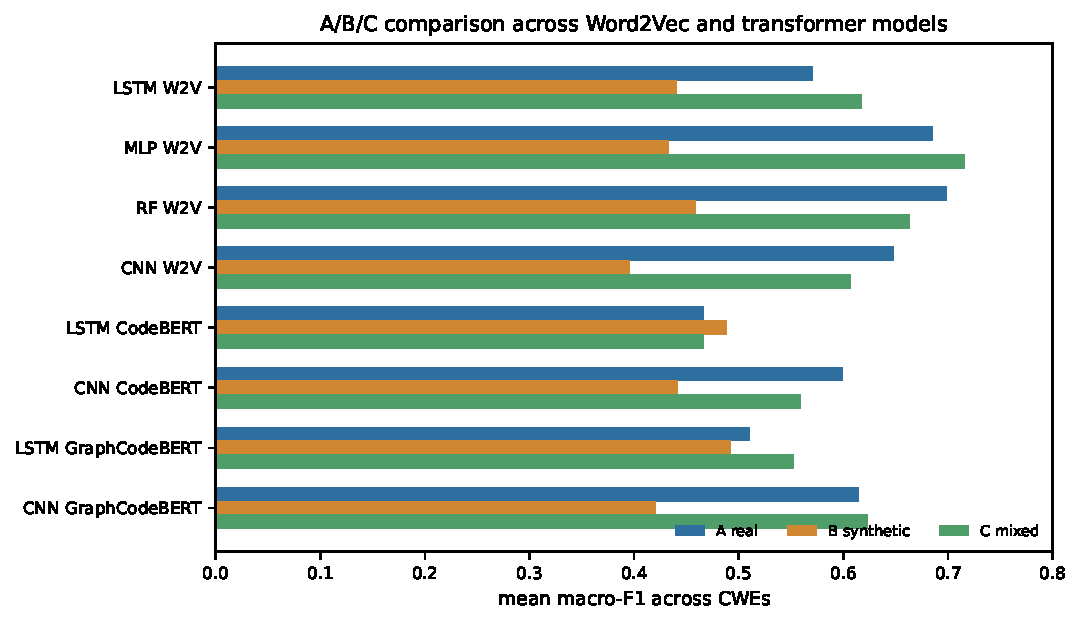
\includegraphics[width=\linewidth]{abc_macro_f1.pdf}
\caption{Mean macro-F1 across the seven CWEs on the same held-out real VUDENC test split.}
\label{fig:abc}
\end{figure}

\begin{table}[t]
\centering
\caption{Mean macro-F1 by model and data condition.}
\label{tab:main-results}
\begin{tabular}{lccc}
\toprule
Model & A: Real & B: Synthetic & C: Combined \\
\midrule
LSTM & 0.5407 & 0.4289 & 0.5605 \\
MLP & 0.6463 & 0.3577 & 0.6421 \\
Random Forest & \textbf{0.6618} & 0.3419 & 0.6415 \\
CNN & 0.6124 & 0.3662 & 0.6080 \\
\bottomrule
\end{tabular}
\end{table}

Real-only training was strongest for every model family overall. Random Forest achieved the best mean macro-F1 (0.6618), followed by MLP (0.6463), CNN (0.6124), and LSTM (0.5407). Synthetic-only training was substantially weaker for all models. The combined condition slightly improved LSTM from 0.5407 to 0.5605, but did not improve CNN, MLP, or Random Forest.

Table~\ref{tab:per-cwe} lists the strongest macro-F1 configuration for each CWE. The table should be interpreted with the common real test set in mind: it identifies useful per-CWE patterns, but the small fixed test subsets limit fine-grained conclusions.

\begin{table*}[t]
\centering
\caption{Best macro-F1 configuration per CWE on held-out real VUDENC windows.}
\label{tab:per-cwe}
\begin{tabular}{lccccccc}
\toprule
CWE mode & Command & Path & Redirect & RCE & SQL & XSRF & XSS \\
\midrule
Best model & MLP & MLP & Random Forest & LSTM & Random Forest & Random Forest & Random Forest \\
Condition & C & A & A & C & A & C & A \\
Macro-F1 & 0.6897 & 0.6096 & 0.7308 & 0.6652 & 0.6544 & 0.7040 & 0.6950 \\
\bottomrule
\end{tabular}
\end{table*}

\section{Discussion and Limitations}\label{sec:discussion}
The result answers the research question conservatively. The pipeline can produce a validated, diverse, balanced-at-commit-level synthetic corpus, but the corpus did not replace real VUDENC data for this window-based classification task. The result is not evidence that synthetic data is intrinsically useless. It is evidence that source representation and distribution matching are decisive.

Figure~\ref{fig:labels} exposes the main representation limitation. The real training split contains both clean and vulnerable windows. The synthetic training split contains 496 vulnerable windows and only 17 clean windows. Many generated files are shorter than 200 tokens, so their only source window overlaps the changed vulnerable region. The synthetic-only models therefore learned a positive-skewed decision rule, causing false positives on real clean windows. This explains why some synthetic-only runs show high vulnerable recall but poor macro-F1.

\begin{figure}[t]
\centering
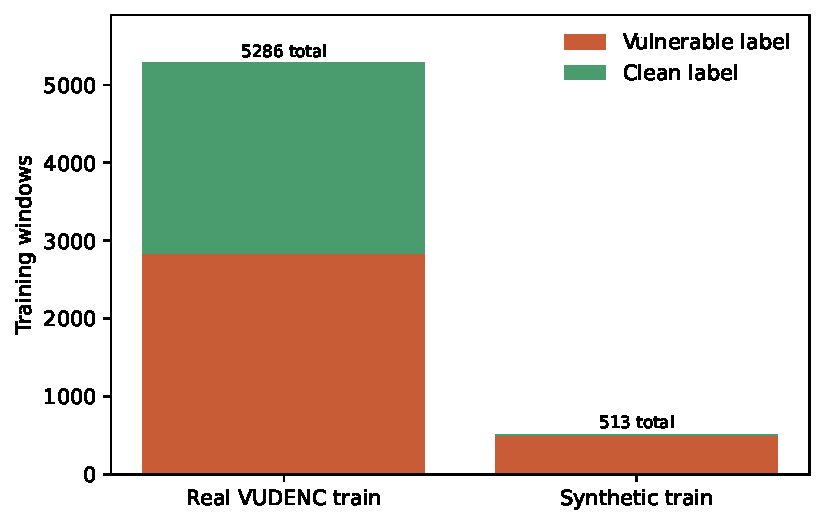
\includegraphics[width=\linewidth]{training_label_distribution.pdf}
\caption{Training-window label distribution. Compact synthetic files produced a severe positive-label skew under source-only VUDENC-style window extraction.}
\label{fig:labels}
\end{figure}

Other threats to validity remain. Static analysis and review improve confidence but do not prove exploitability or production realism. The reviewer is an LLM and can share blind spots with the generator, even when configured independently. The corpus is Python-only and covers seven CWEs, so the results should not be generalized to all languages or weakness types. Finally, the frozen real test split is small for RCE and XSS because VUDENC has fewer commits in these modes.

The next experiment should not merely generate more compact pairs. It should either generate longer modules with explicitly verified clean context or define a paired vulnerable/fixed window task and apply that definition symmetrically to both real and synthetic commits. The second option is more practical, but it changes the task from the original source-only VUDENC window protocol and must be reported explicitly.

\section{Conclusion}
SynVulCommit operationalizes controlled synthetic vulnerability-commit generation with quota-based context coverage, layered validation, reviewer gating, near-duplicate control, sanitized export, and strict dataset verification. It produced 678 accepted Python vulnerability-fix pairs and a frozen 637-pair balanced subset for controlled A/B/C evaluation.

The experiments show a clear result: models trained on real VUDENC data generalize better to held-out real VUDENC windows than models trained only on the present synthetic subset. Adding synthetic data produced a small LSTM improvement but did not improve the other evaluated models. The key limitation was not only generation correctness; it was the mismatch between compact synthetic commits and the 200-token source-window labeling scheme. This finding is useful because it identifies a concrete requirement for future synthetic-data work: generation, validation, and downstream representation must be designed together.

\begin{thebibliography}{12}

\bibitem{vudenc}
Laura Wartschinski, Yannic Noller, Thomas Vogel, Timo Kehrer, and Lars Grunske.
2022.
\newblock VUDENC: Vulnerability Detection with Deep Learning on a Natural Codebase for Python.
\newblock \emph{Information and Software Technology} 144 (2022), 106809.
\newblock https://doi.org/10.1016/j.infsof.2021.106809

\bibitem{vuldeepecker}
Zhen Li, Deqing Zou, Shouhuai Xu, Xinyu Ou, Hai Jin, Sujuan Wang, Zhijun Deng, and Yuyi Zhong.
2018.
\newblock VulDeePecker: A Deep Learning-Based System for Vulnerability Detection.
\newblock In \emph{Proceedings of the Network and Distributed System Security Symposium}.
\newblock https://doi.org/10.14722/ndss.2018.23158

\bibitem{russell2018}
Rebecca Russell, Louis Kim, Lei Hamilton, Tom Lazovich, Jacob Harer, Onur Ozdemir, Paul M. Ellingwood, and Marc McConley.
2018.
\newblock Automated Vulnerability Detection in Source Code Using Deep Representation Learning.
\newblock In \emph{2018 17th IEEE International Conference on Machine Learning and Applications}.
\newblock https://doi.org/10.1109/ICMLA.2018.00120

\bibitem{sysevr}
Zhen Li, Deqing Zou, Shouhuai Xu, Hai Jin, Yawei Zhu, and Zhaoxuan Chen.
2022.
\newblock SySeVR: A Framework for Using Deep Learning to Detect Software Vulnerabilities.
\newblock \emph{IEEE Transactions on Dependable and Secure Computing} 19, 4 (2022), 2244--2258.
\newblock https://doi.org/10.1109/TDSC.2021.3051525

\bibitem{devign}
Yaqin Zhou, Shangqing Liu, Jing Kai Siow, Xiaoning Du, and Yang Liu.
2019.
\newblock Devign: Effective Vulnerability Identification by Learning Comprehensive Program Semantics via Graph Neural Networks.
\newblock In \emph{Advances in Neural Information Processing Systems}.

\bibitem{bigvul}
Jiahao Fan, Yi Li, Shaohua Wang, and Tien N. Nguyen.
2020.
\newblock A C/C++ Code Vulnerability Dataset with Code Changes and CVE Summaries.
\newblock In \emph{Proceedings of the 17th International Conference on Mining Software Repositories}, 508--512.
\newblock https://doi.org/10.1145/3379597.3387501

\bibitem{chakraborty2022}
Saikat Chakraborty, Rahul Krishna, Yangruibo Ding, and Baishakhi Ray.
2022.
\newblock Deep Learning Based Vulnerability Detection: Are We There Yet?
\newblock \emph{IEEE Transactions on Software Engineering} 48, 9 (2022), 3280--3296.
\newblock https://doi.org/10.1109/TSE.2021.3087402

\bibitem{codebert}
Zhangyin Feng, Daya Guo, Duyu Tang, Nan Duan, Xiaocheng Feng, Ming Gong, Linjun Shou, Bing Qin, Ting Liu, Daxin Jiang, and Ming Zhou.
2020.
\newblock CodeBERT: A Pre-Trained Model for Programming and Natural Languages.
\newblock In \emph{Findings of the Association for Computational Linguistics: EMNLP 2020}, 1536--1547.
\newblock https://doi.org/10.18653/v1/2020.findings-emnlp.139

\bibitem{graphcodebert}
Daya Guo, Shuo Ren, Shuai Lu, Zhangyin Feng, Duyu Tang, Shujie Liu, Long Zhou, Nan Duan, Alexey Svyatkovskiy, Shengyu Fu, Michele Tufano, Shao Kun Deng, Colin Clement, and Ming Zhou.
2021.
\newblock GraphCodeBERT: Pre-Training Code Representations with Data Flow.
\newblock In \emph{International Conference on Learning Representations}.

\bibitem{vulberta}
Hazim Hanif and Sergio Maffeis.
2022.
\newblock VulBERTa: Simplified Source Code Pre-Training for Vulnerability Detection.
\newblock In \emph{2022 International Joint Conference on Neural Networks}, 1--8.
\newblock https://doi.org/10.1109/IJCNN55064.2022.9892280

\bibitem{pearce2022}
Hammond Pearce, Baleegh Ahmad, Benjamin Tan, Brendan Dolan-Gavitt, and Ramesh Karri.
2022.
\newblock Asleep at the Keyboard? Assessing the Security of GitHub Copilot's Code Contributions.
\newblock In \emph{2022 IEEE Symposium on Security and Privacy}, 754--768.
\newblock https://doi.org/10.1109/SP46214.2022.9833571

\bibitem{deng2024}
Xiao Deng, Fuyao Duan, Rui Xie, Wei Ye, and Shikun Zhang.
2024.
\newblock Improving Long-Tail Vulnerability Detection Through Data Augmentation Based on Large Language Models.
\newblock In \emph{2024 IEEE International Conference on Software Maintenance and Evolution}, 262--274.
\newblock https://doi.org/10.1109/ICSME58944.2024.00033

\end{thebibliography}

\end{document}
